\chapter{آموزش شناساگر روی داده‌های شبیه‌سازی‌شده}
\label{ch:train}

در این فصل شناساگر ترکیبی کلاسیک و کوانتومی جت‌های \Zbb را روی داده‌هایی که در فصل~\ref{ch:data} خودمان شبیه‌سازی کردیم آموزش می‌دهیم. نخست مجموعه‌های داده و نقش هر کدام را مشخص می‌کنیم. سپس مدل بهینه‌شده را، که آن را \lr{QGNN+} می‌نامیم، با مدل فصل~\ref{ch:tagger} مقایسه می‌کنیم، نتایج آن را می‌آوریم و با شبکه‌های کلاسیک می‌سنجیم، و در پایان خروجی آن را برای جداسازی رویدادهای \ttZ از \ttbb به کار می‌بریم.

\section{مجموعه‌های داده و نقش آنها}
\label{sec:ch3-sets}
چهار مجموعه داده با چهار نقش متفاوت داریم (جدول~\ref{tab:ch3-sets}). مجموعه مرجع \lr{jetImage}، یعنی همان نمونه ۲۰۰۰۰ جتی \Zbos{} در برابر گلوئون که در فصل~\ref{ch:tagger} به کار رفت (بخش~\ref{sec:ch1-data})، مرجع مقایسه با مدل فصل~\ref{ch:tagger} است (پیوست~\ref{app:ch3-first}). نمونه \Zjet در برابر \bbbb همه شناساگرهای جت را آموزش می‌دهد: \lr{QGNN}، شبکه عصبی گرافی کلاسیک، \lr{ParT} و \lr{ParticleNet}. جت‌های \ttZ و \ttbb هرگز در آموزش به کار نمی‌روند و فقط توسط شناساگرها امتیاز می‌گیرند تا ببینیم هر شناساگر چقدر به داده‌های دیگر منتقل می‌شود. در پایان، رویدادهای \ttZ و \ttbb جداکننده رویداد را آموزش می‌دهند. هر شناساگر روی یک جفت جت آموزش می‌بیند. امتیاز شناساگر برای هر جت یک عدد است، و جداکننده رویداد از آن به‌عنوان یک ویژگی اضافه استفاده می‌کند.

\begin{table}[H]
\centering
\caption{مجموعه‌های داده و نقش آنها در آموزش.}
\label{tab:ch3-sets}
\begin{tabular}{p{3.6cm}p{4.2cm}p{7cm}}
\toprule
مجموعه & اندازه & نقش \\
\midrule
\lr{jetImage}: \Zbos{} در برابر گلوئون & ۲۰۰۰۰ جت، همان نمونه فصل~\ref{ch:tagger} & مرجع مقایسه با مدل فصل~\ref{ch:tagger} \\
\Zjet در برابر \bbbb & ۱۹۹۹۲ جت متوازن: ۹۹۹۶ آموزش، ۴۹۹۸ اعتبارسنجی، ۴۹۹۸ آزمون & همه شناساگرها را آموزش می‌دهد \\
جت‌های \ttZ و \ttbb & ۵۰۰۰ جت از هر کدام & فقط امتیازدهی؛ هیچ‌گاه آموزش نمی‌بینند \\
رویدادهای \ttZ و \ttbb & ۴۰۰۰۰ رویداد & جداکننده رویداد (\lr{VQC} یا \lr{BDT}) را روی ۸ ویژگی جت، با امتیاز شناساگر یا بدون آن، آموزش می‌دهند \\
\bottomrule
\end{tabular}
\end{table}

جت‌های \Zjet و \ttZ سیگنال (برچسب ۱) و جت‌های \bbbb و \ttbb پس‌زمینه (برچسب ۰) هستند. تعداد جت‌های برچسب‌دار در هر نمونه چنین است: ۱۳۱۹۷ جت \Zjet، ۱۴۹۳۴ جت \ttZ، ۲۴۳۷۵ جت \bbbb و ۱۳۶۴۸ جت \ttbb. هر مجموعه آموزشی متوازن شده است.

\section{مدل \lr{QGNN+} و تفاوت آن با مدل فصل~\ref{ch:tagger}}
\label{sec:ch3-model}
ساختار کلی مدل همان فصل~\ref{ch:tagger} است: ورودی هر جت ده گره دارد (ده ذره پرانرژی‌تر)، رمزگذار مشترک $160\to128\to64\to4$ برای هر گره یک بردار نهان چهارعددی می‌دهد، گراف ده‌گره‌ای از سه نزدیک‌ترین همسایه در فضای نهان با وزن یال عکس فاصله ساخته می‌شود، و مدار ده‌کیوبیتی با میانگین $\langle Z\rangle$ خروجی می‌دهد. تابع زیان آنتروپی متقاطع دودویی به‌علاوه جمله مولد نویز سینخورن است. مدل روی داده‌های فصل~\ref{ch:data} را با این تغییرها بهینه کردیم (جدول~\ref{tab:ch3-diff}).

\begin{table}[H]
\centering
\caption{تفاوت مدل فصل~\ref{ch:tagger} و \lr{QGNN+}. سایر تنظیم‌ها (بهینه‌ساز \lr{Adam}، تضعیف وزن $10^{-4}$، اندازه دسته ۱۶، ۷۰ دوره، ۳ بذر تصادفی) تغییری نکرده‌اند.}
\label{tab:ch3-diff}
\begin{tabular}{p{3.8cm}p{5.6cm}p{5.6cm}}
\toprule
مورد & مدل فصل~\ref{ch:tagger} & \lr{QGNN+} \\
\midrule
ورودی هر گره & ۱۶۰ عدد (اختلاف با ده همسایه) & ۱۸۱ عدد: ۱۶۰ اختلاف همسایه‌ها، ۱۶ ویژگی مطلق ذره اصلی و ۵ ویژگی سطح جت \\
دراپ‌اوت رمزگذار & \lr{0.3} & \lr{0.1} \\
نرخ یادگیری & \lr{0.008} & \lr{0.003} \\
ساختار مدار & چهار بلوک بارگذاری مجدد، ۲۷۱ پارامتر & دو لایه با بارگذاری هر چهار عدد نهان در هر لایه، ۵۶۲ پارامتر؛ یک لایه هم آزموده شد \\
\bottomrule
\end{tabular}
\end{table}

مدل فصل~\ref{ch:tagger} با ورودی ۱۶۰‌عددی روی این داده‌ها خوب کار نکرد (پیوست~\ref{app:ch3-first}): ورودی فقط قدر مطلق اختلاف هر همسایه با ذره اصلی را نگه می‌داشت و \pt مطلق، انرژی و کمیت‌های سطح جت از آن حذف شده بودند. به همین دلیل به ورودی هر گره ویژگی‌هایی افزودیم. فهرست کامل ورودی شناساگر برای هر گره چنین است:
\begin{itemize}
\item ۱۶۰ عدد: قدر مطلق اختلاف ۱۶ ویژگی ذره اصلی با هر یک از ده نزدیک‌ترین همسایه آن در فضای $(\eta_\mathrm{rel},\varphi_\mathrm{rel})$ (ویژگی‌ها در پیوست~\ref{app:cons} آمده‌اند)؛
\item ۱۶ عدد: خود آن ۱۶ ویژگی ذره اصلی، به‌صورت مطلق؛
\item ۵ عدد: ویژگی‌های سطح جت یعنی جرم، \pt، تعداد ذره‌ها، \lr{girth} و \lr{$p_\mathrm{T}D$}، که روی هر ده گره تکرار می‌شوند.
\end{itemize}
جت‌های \ttZ و \ttbb با همان ۱۸۱ عدد و همان مقیاس‌دهی ساخته می‌شوند. جزئیات آزمایش‌هایی که به این تغییرها انجامید در پیوست~\ref{app:ch3-first} توضیح داده شده است.

\section{نتایج \lr{QGNN+}}
\label{sec:ch3-qgnnp}
با دراپ‌اوت \lr{0.1} و نرخ یادگیری \lr{0.003} مدل پایدار آموزش می‌بیند: \lr{AUC} آزمون روی \Zjet در برابر \bbbb برابر $0.866\pm0.001$ با دو لایه و $0.869\pm0.001$ با یک لایه است، هر کدام با ۳ بذر تصادفی (شکل~\ref{fig:ch3-jetroc}). رد پس‌زمینه در کارایی سیگنال ۶۰، ۸۰ و ۹۰ درصد در جدول~\ref{tab:ch3-rej} آمده است.

\begin{figure}[H]
\centering
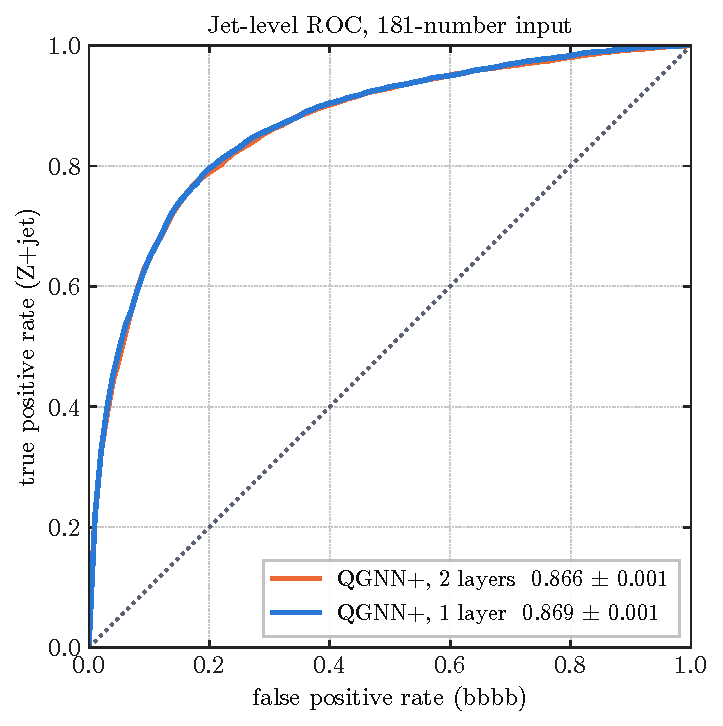
\includegraphics[width=0.6\textwidth]{figs/ch3_jet_roc.pdf}
\caption{منحنی \lr{ROC} آزمون \lr{QGNN+} روی \Zjet در برابر \bbbb (۳ بذر تصادفی، نوار \lr{$\pm$}یک انحراف معیار).}
\label{fig:ch3-jetroc}
\end{figure}

\section{مقایسه \lr{QGNN+} با مدل‌های کلاسیک}
\label{sec:ch3-compare}
\lr{QGNN+} عملکردی هم‌سطح مدل‌های کلاسیک مشابه دارد. شبکه گرافی کلاسیک با همان رمزگذار و گراف، که به‌جای مدار از انتقال پیام استفاده می‌کند، با تنظیمات پیش‌فرض \lr{AUC} برابر \lr{0.861} می‌دهد؛ وقتی نرخ یادگیری و دراپ‌اوت آن مانند \lr{QGNN+} باشد به $0.8669\pm0.0009$ می‌رسد، در برابر $0.8665\pm0.0007$ برای \lr{QGNN+} با دو لایه. امتیاز دو مدل روی جت‌های یکسان با ضریب \lr{0.984} همبسته است. این هم‌سطحی در داده کم نیز دیده می‌شود: \lr{QGNN+} و شبکه کلاسیک از ۱۰۰ تا ۳۰۰۰ جت آموزشی در محدوده پراکندگی بذرهای تصادفی با هم برابرند (برای نمونه \lr{0.667} در برابر \lr{0.654} با ۱۰۰ جت و \lr{0.857} در برابر \lr{0.852} با ۳۰۰۰ جت؛ با ۲ بذر تصادفی برای \lr{QGNN+} در ۳۰۰۰ جت؛ شکل~\ref{fig:ch3-dataeff}). یعنی مدار کوانتومی با ۵۶۲ پارامتر به همان کیفیت شبکه کلاسیک می‌رسد.

\begin{figure}[H]
\centering
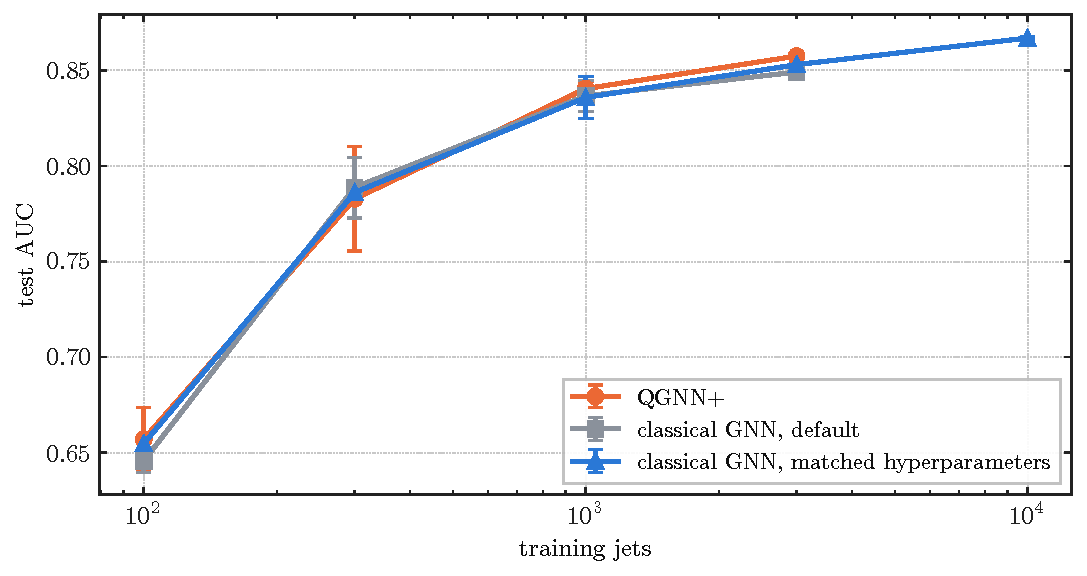
\includegraphics[width=0.7\textwidth]{figs/ch3_dataeff.pdf}
\caption{\lr{AUC} آزمون بر حسب تعداد جت‌های آموزشی (محور افقی لگاریتمی)؛ نوار خطا انحراف معیار روی بذرهای تصادفی است.}
\label{fig:ch3-dataeff}
\end{figure}

شبکه‌های \lr{ParT} و \lr{ParticleNet} را هم خودمان روی همین جت‌ها دوباره آموزش دادیم (جدول~\ref{tab:ch3-final}). با همان ورودی \lr{QGNN+}، یعنی ده گره با ۱۸۱ عدد، به \lr{0.840} و \lr{0.849} می‌رسند و \lr{QGNN+} از هر دو بهتر است. با ذره‌های خام (تا ۱۲۸ ذره با ۷ ویژگی) به \lr{0.883} و \lr{0.886} می‌رسند، یعنی ورودی ذره‌های خام تعیین‌کننده است. این دو شبکه برای ورودی ۱۸۱‌عددی تنظیم نشده‌اند (شکل~\ref{fig:ch3-cmp}).

\begin{figure}[H]
\centering
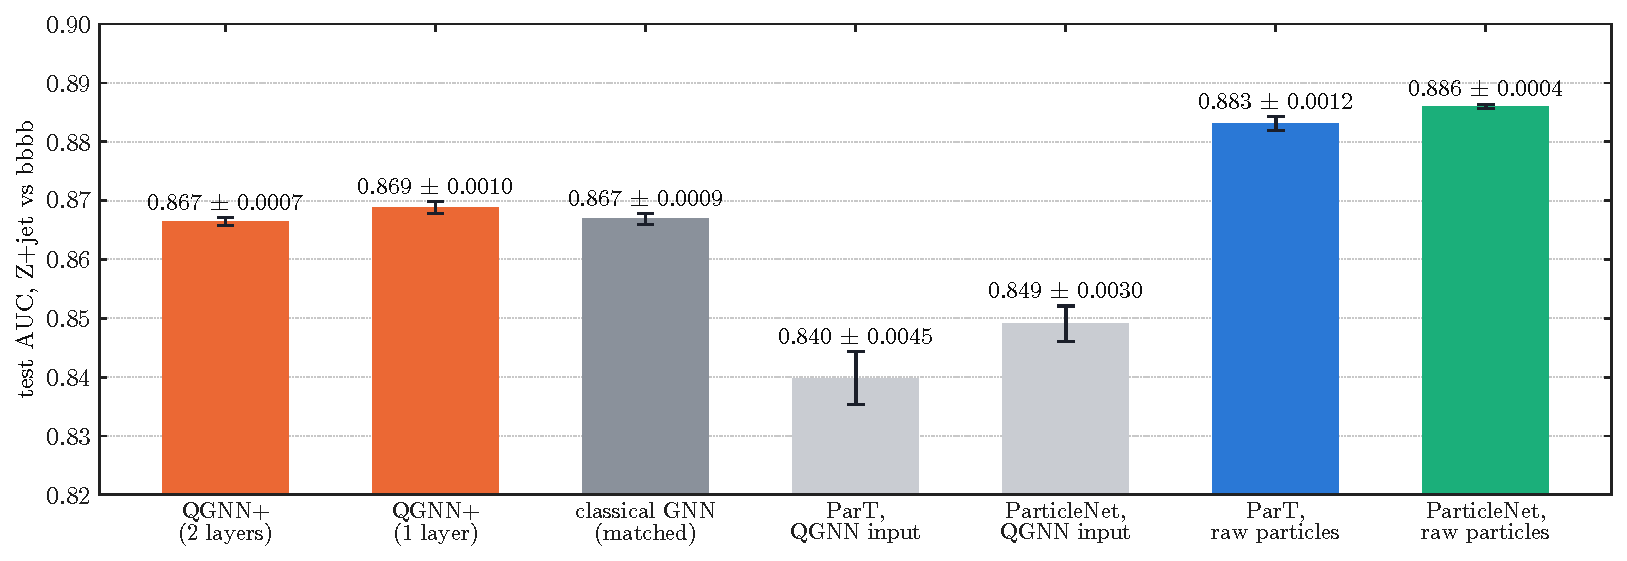
\includegraphics[width=\textwidth]{figs/ch3_cmp.pdf}
\caption{مقایسه \lr{AUC} آزمون مدل‌ها روی \Zjet در برابر \bbbb با ورودی جدید؛ نوار خطا انحراف معیار روی بذرهای تصادفی است.}
\label{fig:ch3-cmp}
\end{figure}

\begin{table}[H]
\centering
\caption{\lr{AUC} آزمون روی \Zjet در برابر \bbbb با ورودی جدید؛ \lr{$\pm$} انحراف معیار روی بذرهای تصادفی.}
\label{tab:ch3-final}
\begin{tabular}{lc}
\toprule
مدل & \lr{AUC} \\
\midrule
\lr{BDT} & \lr{0.865} \\
\lr{MLP} & \lr{0.851} \\
شبکه گرافی کلاسیک، پیش‌فرض & $0.861\pm0.007$ \\
شبکه گرافی کلاسیک، تنظیم یکسان با \lr{QGNN+} & $0.8669\pm0.0009$ \\
\lr{QGNN+}، دو لایه & $0.8665\pm0.0007$ \\
\lr{QGNN+}، یک لایه & $0.8688\pm0.001$ \\
\lr{ParT}، ده گره (ورودی یکسان) & $0.8398\pm0.0045$ \\
\lr{ParticleNet}، ده گره (ورودی یکسان) & $0.8491\pm0.0030$ \\
\lr{ParT}، ذره‌های خام & $0.8831\pm0.0012$ \\
\lr{ParticleNet}، ذره‌های خام & $0.8860\pm0.0004$ \\
\bottomrule
\end{tabular}
\end{table}

\section{جداسازی رویدادهای \ttZ از \ttbb}
\label{sec:ch3-transfer}
شناساگر جت را برای جداسازی رویدادهای \ttZ از \ttbb در دو آرایش به کار می‌بریم، و جداکننده رویداد در این دو آرایش داده‌های متفاوتی می‌خواند. در آرایش نخست (بخش~\ref{sub:ch3-jetfeat}) جداکننده فقط چند ویژگی ساده از دو جت اول رویداد را می‌گیرد و امتیاز شناساگر را به‌عنوان یک ویژگی اضافه می‌کند. در آرایش دوم (بخش~\ref{sec:ch3-evqgnn}) همه اجزای رویداد، یعنی هفت جت، دو لپتون و \lr{MET}، به جداکننده داده می‌شوند و امتیاز شناساگر به جت‌های اول و دوم افزوده می‌شود. جدول~\ref{tab:ch3-inputs} ورودی هر آرایش را کنار هم می‌گذارد.

\begin{table}[H]
\centering
\caption{ورودی جداکننده رویداد در دو آرایش.}
\label{tab:ch3-inputs}
\small
\begin{tabular}{p{2.6cm}p{6.4cm}p{6.4cm}}
\toprule
 & بخش~\ref{sub:ch3-jetfeat}: ویژگی‌های دو جت اول & بخش~\ref{sec:ch3-evqgnn}: ده شیء رویداد \\
\midrule
جداکننده‌ها & \lr{VQC} و \lr{BDT} & \lr{QGNN} رویدادی (مدار کوانتومی)، کنترل کلاسیک آن، چهار مدل کلاسیک (\lr{MLP}، شبکه گرافی، شبیه \lr{ParticleNet}، ترنسفورمر) و \lr{BDT} \\
ورودی اصلی & ۸ عدد: \pt، $\eta$ و جرم هر یک از دو جت اول، تعداد جت‌های رویداد و جرم ناوردای دو جت اول ($M_{jj}$) & هفت جت، دو لپتون و \lr{MET}، هر کدام یک گره. برای هر گره: $\log(1+p_\mathrm{T})$، $\eta$، $\cos\varphi$، $\sin\varphi$، $\log(1+m)$ (برای لپتون و \lr{MET} جرم صفر است) و نوع شیء (جت، لپتون یا \lr{MET}). هر ویژگی برای هر جایگاه جداگانه با تبدیل چندکی به توزیع نرمال برده می‌شود \\
ورودی‌های دیگر & اختیاری: جرم \lr{soft-drop} جت اول (\lr{msd0}) & ویژگی‌های سراسری رویداد: $\log(1+H_\mathrm{T})$، تعداد جت‌ها تقسیم بر ۱۰ و تعداد لپتون‌ها؛ برای \lr{QGNN} رویدادی و کنترل کلاسیک آن، شماره جایگاه هر گره (رتبه جت، لپتون یا \lr{MET}) \\
امتیاز شناساگر & اختیاری: امتیاز \lr{QGNN+} جت اول به‌عنوان یک ورودی دیگر & اختیاری: امتیاز جت اول و جت دوم، به‌همراه نشانگر وجود امتیاز، روی گره همان جت؛ امتیاز از \lr{QGNN+}، شبکه گرافی کلاسیک، \lr{ParT} یا \lr{ParticleNet} \\
\lr{BDT} & همان ۸ تا ۱۰ ورودی & ۴۱ ویژگی: \pt، $\eta$، $\varphi$ و جرم هر هفت جت، \pt، $\eta$، $\varphi$ و انرژی هر دو لپتون، \pt و $\varphi$ مربوط به \lr{MET}، تعداد جت‌ها، تعداد لپتون‌ها و $H_\mathrm{T}$، و در صورت وجود امتیاز شناساگر \\
رویدادهای آزمون & رویدادهایی که جت اولشان امتیاز دارد & رویدادهایی که جت اولشان امتیاز دارد: ۱۸۰۴۶ رویداد آموزش و ۶۰۱۲ رویداد آزمون \\
\bottomrule
\end{tabular}
\end{table}

\subsection{جداکننده روی ویژگی‌های دو جت اول}
\label{sub:ch3-jetfeat}
شناساگر فقط روی \Zjet در برابر \bbbb آموزش دیده است و هیچ جت \ttZ یا \ttbb را ندیده است، ولی می‌توانیم آن را روی جت‌های این رویدادها اجرا کنیم و ببینیم تا چه اندازه جت ناشی از \Zbos{} را از جت \bbbb در رویدادهای \ttbb جدا می‌کند. برای سنجش این کار، به جت اول هر رویداد آزمون یک امتیاز می‌دهیم و فقط با همین امتیاز، به‌کمک یک \lr{BDT}، رویدادهای \ttZ و \ttbb را جدا می‌کنیم. این کار فقط روی رویدادهایی ممکن است که جت اولشان امتیاز دارد، که ۷۵ درصد رویدادها هستند. امتیاز \lr{QGNN+} در این حالت \lr{AUC} برابر \lr{0.793} می‌دهد و امتیاز شبکه گرافی کلاسیک \lr{0.787}، یعنی شناساگری که روی جت‌های \Zjet آموزش دیده تا حد خوبی به جت‌های رویدادهای \ttZ منتقل می‌شود. امتیاز جت دوم رویداد جداسازی ضعیف‌تری می‌دهد و \lr{QGNN+} با آن \lr{AUC} برابر \lr{0.654} می‌دهد. برای دانستن اینکه امتیاز شناساگر چه چیزی را اندازه می‌گیرد، همبستگی آن را با کمیت‌های ساده جت سنجیده‌ایم: ضریب همبستگی امتیاز با جرم جت \lr{$-0.42$}، با تعداد مؤلفه‌ها \lr{$-0.58$} و با جرم \lr{soft-drop} جت اول، \lr{msd0}، برابر \lr{$-0.28$} است. پس امتیاز شناساگر تا اندازه‌ای نماینده جرم جت است و فقط به آن محدود نمی‌شود، چون فراتر از \lr{msd0} حدود \lr{0.03} به \lr{AUC} جداکننده رویداد می‌افزاید (جدول~\ref{tab:ch3-event}).

برای رسیدن به هدف نهایی، یک جداکننده رویداد روی ۴۰۰۰۰ رویداد \ttZ و \ttbb آموزش می‌دهیم. چهار مجموعه ورودی می‌سنجیم (جدول~\ref{tab:ch3-inputs}): ۸ ویژگی جت، ۸ ویژگی به‌علاوه \lr{msd0}، ۸ ویژگی به‌علاوه امتیاز \lr{QGNN+}، و هر سه با هم. این ویژگی‌ها لپتون و \lr{MET} را شامل نمی‌شوند؛ آن‌ها در بخش~\ref{sec:ch3-evqgnn} وارد می‌شوند.

\textbf{جداکننده‌ها.} مدار کوانتومی وردشی (\lr{VQC}) به ازای هر ورودی یک کیوبیت دارد، پس ۸ تا ۱۰ کیوبیت. \pt، جرم‌ها و $M_{jj}$ با $\log(1+x)$ تبدیل می‌شوند، سپس هر ورودی با میانگین و انحراف معیار رویدادهای آموزش به میانگین صفر و انحراف معیار یک برده می‌شود و با زاویه $2\arctan(x)$ در چرخش‌های مدار بارگذاری می‌شوند. مدار ۴ لایه دارد و با بهینه‌ساز \lr{Adam} (نرخ یادگیری \lr{0.02}، اندازه دسته ۲۵۶، ۴۰ دوره) و ۳ بذر تصادفی آموزش می‌بیند. \lr{BDT} درخت تصمیم تقویت‌شده با گرادیان (\lr{HistGradientBoosting} در \lr{scikit-learn}) با ۳۰۰ تکرار و نرخ یادگیری \lr{0.05} است که همان ورودی‌ها را بدون تبدیل می‌خواند، با ۳ بذر تصادفی.

\textbf{نتایج.} فقط با ۸ ویژگی جت، \lr{AUC} برابر \lr{0.758} برای \lr{VQC} و \lr{0.764} برای \lr{BDT} است. با افزودن امتیاز \lr{QGNN+} این مقدار به \lr{0.831} و \lr{0.835} می‌رسد، یعنی حدود \lr{0.07} بیشتر. افزودن \lr{msd0} به ۸ ویژگی \lr{AUC} را به \lr{0.815} و \lr{0.825} می‌رساند، و با \lr{msd0} و امتیاز با هم به \lr{0.842} و \lr{0.852} می‌رسد. سهم امتیاز شناساگر فراتر از \lr{msd0} در هر دو جداکننده حدود \lr{0.03} است (جدول~\ref{tab:ch3-event}).

\begin{table}[H]
\centering
\caption{\lr{AUC} آزمون جداکننده رویداد \ttZ در برابر \ttbb. هر مقدار میانگین ۳ بذر تصادفی است (۲ بذر تصادفی برای \lr{VQC} با \lr{msd0} و امتیاز).}
\label{tab:ch3-event}
\begin{tabular}{lcc}
\toprule
ویژگی‌ها & \lr{VQC} & \lr{BDT} \\
\midrule
ویژگی‌های جت (۸ ویژگی) & \lr{0.758} & \lr{0.764} \\
با امتیاز \lr{QGNN+} & \lr{0.831} & \lr{0.835} \\
با \lr{msd0} & \lr{0.815} & \lr{0.825} \\
با \lr{msd0} و امتیاز & \lr{0.842} & \lr{0.852} \\
\bottomrule
\end{tabular}
\end{table}

منحنی‌های \lr{ROC} دو جداکننده در شکل~\ref{fig:ch3-evroc} آمده است. برای مقایسه در نقطه‌های کاری، رد پس‌زمینه، یعنی وارون نرخ مثبت کاذب، در کارایی سیگنال \lr{60}، \lr{80} و \lr{90} درصد در جدول~\ref{tab:ch3-rej} آمده است. این مقدارها از منحنی \lr{ROC} میانگین بذرهای تصادفی محاسبه شده‌اند. بازه \lr{VQC} از جابه‌جا کردن منحنی به اندازه \lr{$\pm$}یک انحراف معیار روی بذرهای تصادفی، و بازه \lr{BDT} از نوار بوت‌استرپ ۶۸ درصد روی رویدادهای آزمون به دست آمده است.

\begin{figure}[H]
\centering
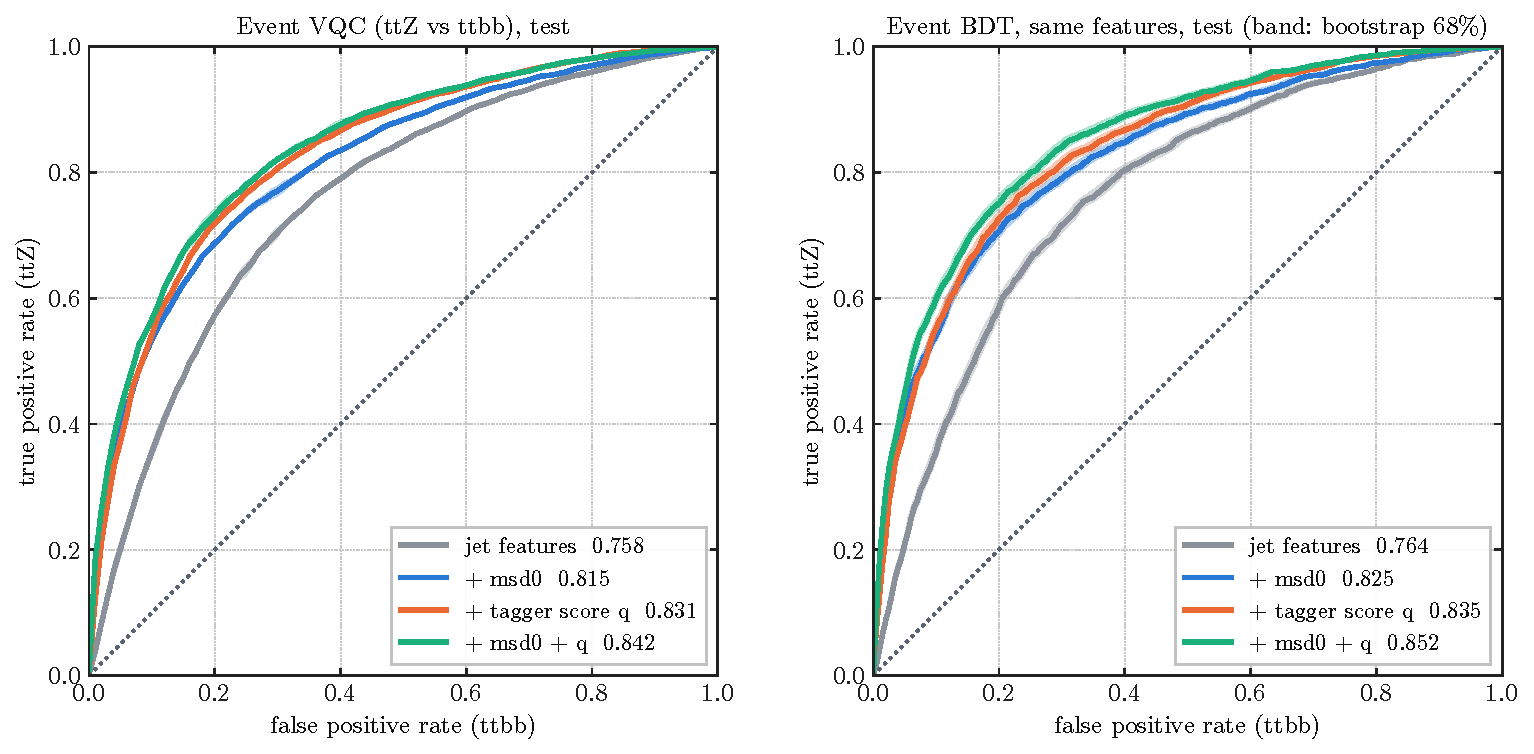
\includegraphics[width=\textwidth]{figs/ch3_event_roc.pdf}
\caption{منحنی \lr{ROC} آزمون جداکننده رویداد \ttZ در برابر \ttbb: \lr{VQC} (چپ) و \lr{BDT} (راست) با مجموعه‌های مختلف ویژگی. نوار: \lr{$\pm$}یک انحراف معیار روی بذرهای تصادفی برای \lr{VQC}، و بوت‌استرپ ۶۸ درصد روی رویدادهای آزمون برای \lr{BDT}.}
\label{fig:ch3-evroc}
\end{figure}

\begin{table}[H]
\centering
\caption{رد پس‌زمینه (وارون نرخ مثبت کاذب) در کارایی سیگنال ثابت. بخش بالا: \lr{QGNN+} روی جت‌ها (\Zjet در برابر \bbbb)؛ بخش‌های پایین: جداکننده‌های رویداد (\ttZ در برابر \ttbb).}
\label{tab:ch3-rej}
\begin{tabular}{lccc}
\toprule
مدل & \lr{60\%} & \lr{80\%} & \lr{90\%} \\
\midrule
\lr{QGNN+}، دو لایه & $12.1^{+0.3}_{-0.2}$ & $4.6^{+0.1}_{-0.1}$ & $2.5^{+0.0}_{-0.0}$ \\
\lr{QGNN+}، یک لایه & $12.1^{+0.1}_{-0.1}$ & $4.9^{+0.1}_{-0.1}$ & $2.6^{+0.0}_{-0.0}$ \\
\midrule
جداکننده \lr{VQC}، ویژگی‌های جت & $4.6^{+0.1}_{-0.1}$ & $2.4^{+0.0}_{-0.0}$ & $1.7^{+0.0}_{-0.0}$ \\
\lr{VQC}، با امتیاز & $8.0^{+0.1}_{-0.1}$ & $3.4^{+0.1}_{-0.1}$ & $2.1^{+0.0}_{-0.0}$ \\
\lr{VQC}، با \lr{msd0} & $7.3^{+0.2}_{-0.2}$ & $2.9^{+0.1}_{-0.0}$ & $1.8^{+0.0}_{-0.0}$ \\
\lr{VQC}، با \lr{msd0} و امتیاز & $8.8^{+0.1}_{-0.1}$ & $3.7^{+0.0}_{-0.0}$ & $2.2^{+0.0}_{-0.0}$ \\
جداکننده \lr{BDT}، ویژگی‌های جت & $4.9^{+0.2}_{-0.2}$ & $2.5^{+0.1}_{-0.1}$ & $1.7^{+0.0}_{-0.0}$ \\
\lr{BDT}، با امتیاز & $8.2^{+0.5}_{-0.5}$ & $3.5^{+0.2}_{-0.1}$ & $2.1^{+0.1}_{-0.1}$ \\
\lr{BDT}، با \lr{msd0} & $8.1^{+0.5}_{-0.4}$ & $3.2^{+0.2}_{-0.1}$ & $1.9^{+0.1}_{-0.1}$ \\
\lr{BDT}، با \lr{msd0} و امتیاز & $10.0^{+0.6}_{-0.6}$ & $4.0^{+0.2}_{-0.2}$ & $2.3^{+0.1}_{-0.1}$ \\
\bottomrule
\end{tabular}

\end{table}

\subsection{جداکننده روی ده شیء رویداد}
\label{sec:ch3-evqgnn}
تا اینجا امتیاز شناساگر جت را به‌عنوان یک ویژگی به جداکننده رویداد (\lr{VQC} یا \lr{BDT}) داده‌ایم. در آخرین مرحله همان مدار ده‌کیوبیتی را مستقیماً روی رویداد به کار بردیم: هر رویداد به ده شیء تبدیل می‌شود (هفت جت، دو لپتون و \lr{MET}) و هر شیء یک گره و یک کیوبیت است. ویژگی هر شیء $\log(1+p_\mathrm{T})$، $\eta$، $\cos\varphi$، $\sin\varphi$، $\log(1+m)$، نوع شیء و شماره جایگاه آن است، و برای جت‌ها در صورت وجود امتیاز شناساگر و نشانگر وجود آن به آن افزوده می‌شود. پیش از ورود به مدل، هر ویژگی هر گره (برای هر جایگاه جداگانه) با تبدیل چندکی (\lr{quantile transform}) به توزیع نرمال برده می‌شود و ویژگی‌های سراسری با میانگین و انحراف معیار نرمال‌سازی می‌شوند؛ هر دو تبدیل فقط روی رویدادهای آموزش برازش می‌شوند. رمزگذار کلاسیک هر شیء را به چهار عدد نهان می‌برد، گراف از سه نزدیک‌ترین همسایه در فضای نهان ساخته می‌شود، و مدار همان مدار بخش~\ref{sec:ch3-model} است؛ خروجی میانگین $\langle Z\rangle$ روی کیوبیت‌های موجود است. آموزش با بهینه‌ساز \lr{Adam}، اندازه دسته ۱۲۸، دراپ‌اوت \lr{0.1}، تا ۴۰ دوره با توقف زودهنگام (شکیبایی ۸ دوره) و نرخ یادگیری \lr{0.001} یا \lr{0.003} (انتخاب‌شده با اعتبارسنجی) انجام می‌شود، با ۳ بذر تصادفی. نمونه شامل رویدادهایی است که جت اول آنها امتیاز دارد: ۱۸۰۴۶ رویداد آموزش و ۶۰۱۲ رویداد آزمون. «\lr{AUC} گروهی» یعنی \lr{AUC} میانگین امتیاز سه بذر تصادفی، و بازه داخل کروشه بازه اطمینان ۹۵ درصد به روش بوت‌استرپ روی رویدادهای آزمون است. برای هر مدل کوانتومی یک کنترل کلاسیک داریم که همان رمزگذار و گراف را دارد و به‌جای مدار از انتقال پیام کلاسیک استفاده می‌کند، و چهار مدل کلاسیک عمومی (\lr{MLP}، شبکه گرافی، شبیه \lr{ParticleNet} و ترنسفورمر) روی همان ده شیء. یک \lr{BDT} هم روی همان رویدادها آموزش دیده که ۴۱ ویژگی می‌خواند: \pt، $\eta$، $\varphi$ و جرم هر هفت جت، \pt، $\eta$، $\varphi$ و انرژی هر دو لپتون، \pt و $\varphi$ مربوط به \lr{MET}، تعداد جت‌ها، تعداد لپتون‌ها و \lr{$H_\mathrm{T}$}، و در صورت وجود امتیاز شناساگر.

\textbf{اثر امتیاز شناساگر.} بدون امتیاز، مدل کوانتومی به \lr{AUC} برابر \lr{0.751} می‌رسد. با افزودن امتیاز \lr{QGNN+} به \lr{0.831} می‌رسد، یعنی افزایشی برابر $+0.080$ با بازه $[+0.070,+0.089]$ (جدول~\ref{tab:ch3-ev1} و شکل~\ref{fig:ch3-evroc2}). امتیاز دو شبکه دیگر که روی ورودی \lr{QGNN+} آموزش دیده‌اند (\lr{ParT} و \lr{ParticleNet}) و امتیاز شبکه گرافی کلاسیک نتیجه‌ای تقریباً یکسان می‌دهند (\lr{0.827} تا \lr{0.831}). امتیاز شبکه‌هایی که روی ذره‌های خام آموزش دیده‌اند بیشتر کمک می‌کند: \lr{0.853} با \lr{ParT} و \lr{0.860} با \lr{ParticleNet}. پس سهم امتیاز را اطلاعات ورودی شناساگر تعیین می‌کند و نه نوع مدل (شکل~\ref{fig:ch3-evtags}).

\begin{table}[H]
\centering
\caption{\lr{AUC} گروهی آزمون برای جداسازی رویدادهای \ttZ از \ttbb بر حسب امتیاز شناساگر جت اول. داخل کروشه بازه اطمینان ۹۵ درصد؛ «افزایش» نسبت به همان مدل بدون امتیاز است.}
\label{tab:ch3-ev1}
\small
\begin{tabular}{lcccc}
\toprule
 & \multicolumn{2}{c}{\lr{QGNN} رویدادی} & \multicolumn{2}{c}{کنترل کلاسیک (بدون مدار)} \\
\cmidrule(lr){2-3}\cmidrule(lr){4-5}
امتیاز ورودی & \lr{AUC} & افزایش نسبت به بدون امتیاز & \lr{AUC} & افزایش \\
\midrule
بدون امتیاز شناساگر & $0.751\,[0.739,\,0.762]$ & --- & $0.762\,[0.750,\,0.774]$ & --- \\
امتیاز \lr{QGNN+} & $0.831\,[0.820,\,0.840]$ & $+0.080\,[+0.070,\,+0.089]$ & $0.837\,[0.827,\,0.847]$ & $+0.075\,[+0.065,\,+0.084]$ \\
امتیاز شبکه گرافی کلاسیک & $0.827\,[0.816,\,0.837]$ & $+0.076\,[+0.066,\,+0.086]$ & $0.836\,[0.825,\,0.846]$ & $+0.073\,[+0.064,\,+0.082]$ \\
امتیاز \lr{ParT}، ورودی \lr{QGNN+} & $0.829\,[0.818,\,0.839]$ & $+0.078\,[+0.068,\,+0.088]$ & $0.837\,[0.827,\,0.847]$ & $+0.075\,[+0.065,\,+0.084]$ \\
امتیاز \lr{ParticleNet}، ورودی \lr{QGNN+} & $0.831\,[0.820,\,0.841]$ & $+0.080\,[+0.070,\,+0.090]$ & $0.835\,[0.824,\,0.845]$ & $+0.073\,[+0.063,\,+0.082]$ \\
امتیاز \lr{ParT}، ذره‌های خام & $0.853\,[0.843,\,0.862]$ & $+0.102\,[+0.092,\,+0.112]$ & $0.863\,[0.854,\,0.872]$ & $+0.101\,[+0.091,\,+0.111]$ \\
امتیاز \lr{ParticleNet}، ذره‌های خام & $0.860\,[0.851,\,0.869]$ & $+0.109\,[+0.099,\,+0.120]$ & $0.865\,[0.855,\,0.873]$ & $+0.102\,[+0.093,\,+0.112]$ \\
\bottomrule
\end{tabular}

\end{table}

\begin{figure}[H]
\centering
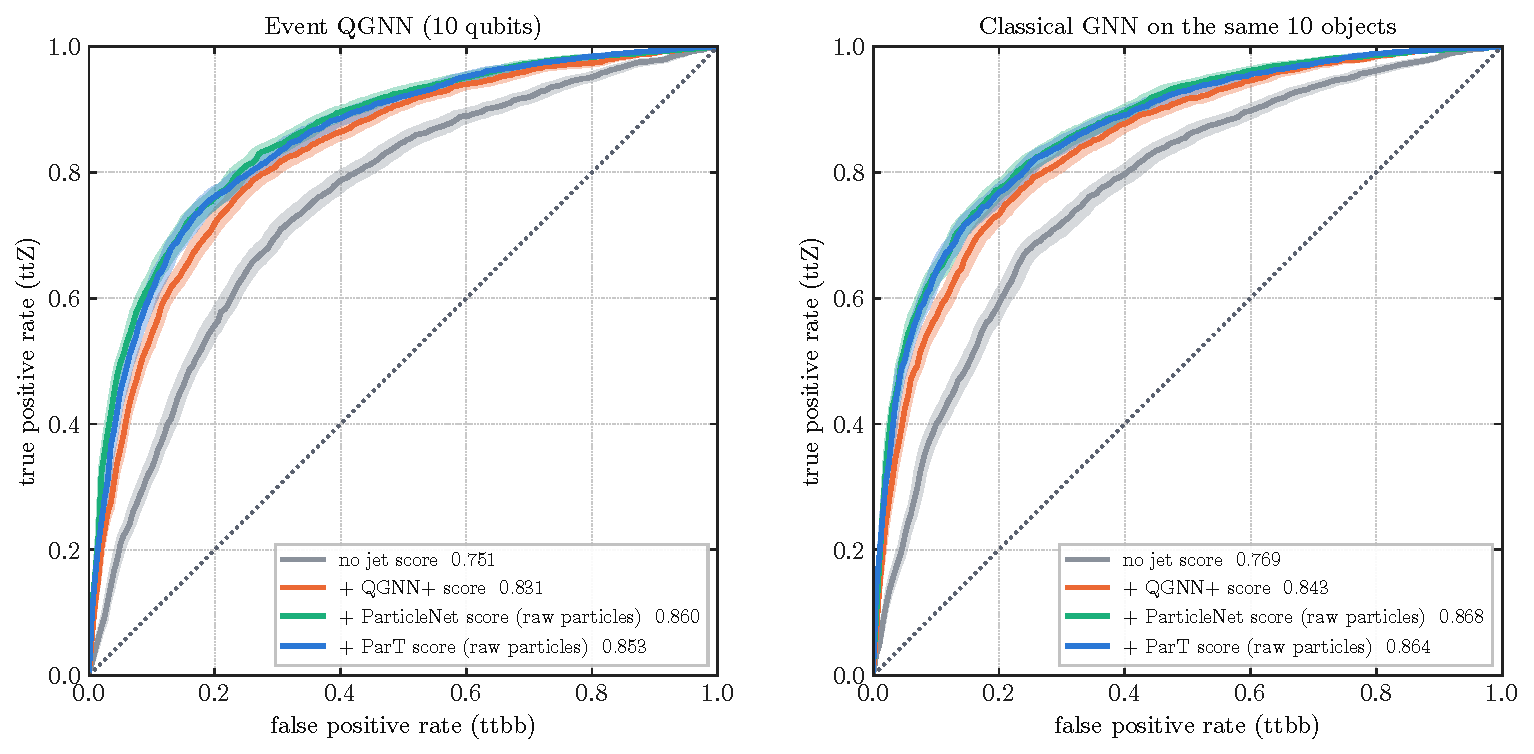
\includegraphics[width=\textwidth]{figs/ch3_ev_roc.pdf}
\caption{منحنی \lr{ROC} آزمون جداکننده رویداد روی ده شیء: \lr{QGNN} رویدادی (چپ) و شبکه گرافی کلاسیک (راست)، بدون امتیاز و با امتیاز سه شناساگر جت. نوار: بازه اطمینان ۹۵ درصد (بوت‌استرپ).}
\label{fig:ch3-evroc2}
\end{figure}

\begin{figure}[H]
\centering
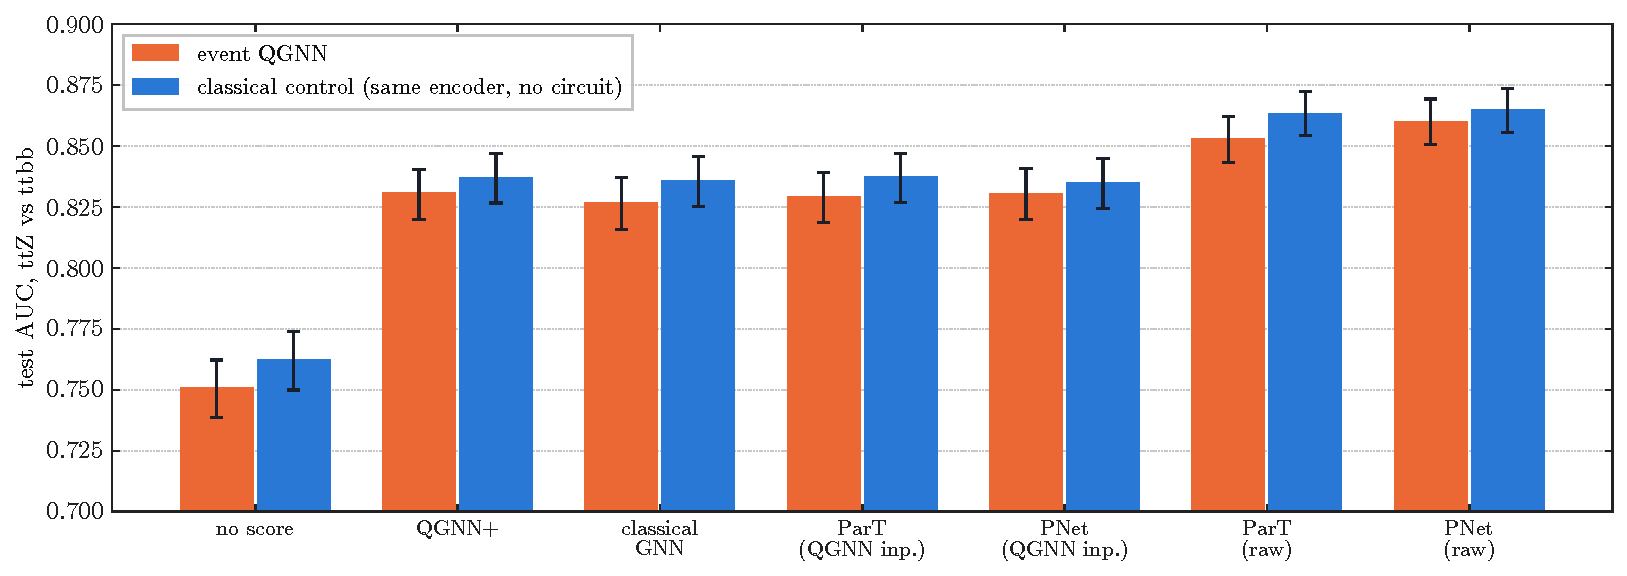
\includegraphics[width=\textwidth]{figs/ch3_ev_tags.pdf}
\caption{\lr{AUC} گروهی آزمون بر حسب امتیاز ورودی، برای مدل کوانتومی و کنترل کلاسیک آن؛ میله خطا بازه اطمینان ۹۵ درصد است.}
\label{fig:ch3-evtags}
\end{figure}

\textbf{مقایسه با مدل‌های کلاسیک.} مدار کوانتومی در هیچ‌یک از حالت‌ها برتری ندارد (جدول~\ref{tab:ch3-ev1} و~\ref{tab:ch3-ev3}). بدون امتیاز، \lr{QGNN} رویدادی \lr{0.751} می‌دهد، کنترل کلاسیک \lr{0.762} و مدل‌های کلاسیک عمومی و \lr{BDT} \lr{0.758} تا \lr{0.777}. با امتیاز \lr{QGNN+}، مدل کوانتومی \lr{0.831} و کنترل کلاسیک \lr{0.837} می‌دهد و مدل‌های کلاسیک عمومی و \lr{BDT} \lr{0.841} تا \lr{0.846}. با امتیاز \lr{ParT} روی ذره‌های خام این مقدارها \lr{0.853}، \lr{0.863} و \lr{0.861} تا \lr{0.869} است (\lr{0.870} تا \lr{0.872} با امتیاز \lr{ParticleNet}). اختلاف مدل کوانتومی با بهترین مدل کلاسیک حدود \lr{0.01} تا \lr{0.02} به زیان مدل کوانتومی است و بازه‌های اطمینان آنها هم‌پوشانی دارند.

\begin{table}[H]
\centering
\caption{\lr{AUC} گروهی آزمون مدل‌های رویدادی روی ده شیء (\lr{BDT}: ۴۱ ویژگی)، بر حسب امتیاز ورودی؛ بازه اطمینان ۹۵ درصد در کروشه.}
\label{tab:ch3-ev3}
\small
\begin{tabular}{lcccc}
\toprule
مدل رویدادی & بدون امتیاز & امتیاز \lr{QGNN+} & \lr{ParT}، ذره‌های خام & \lr{ParticleNet}، ذره‌های خام \\
\midrule
\lr{BDT} (۴۱ ویژگی) & $0.769\,[0.758,\,0.782]$ & $0.841\,[0.832,\,0.852]$ & $0.867\,[0.857,\,0.875]$ & $0.870\,[0.861,\,0.879]$ \\
\midrule
شبکه چندلایه (\lr{MLP}) & $0.758\,[0.747,\,0.771]$ & $0.841\,[0.832,\,0.852]$ & $0.861\,[0.852,\,0.871]$ & $0.862\,[0.853,\,0.871]$ \\
شبکه گرافی & $0.769\,[0.758,\,0.781]$ & $0.843\,[0.834,\,0.854]$ & $0.864\,[0.855,\,0.872]$ & $0.868\,[0.859,\,0.877]$ \\
شبیه \lr{ParticleNet} & $0.770\,[0.759,\,0.783]$ & $0.845\,[0.835,\,0.855]$ & $0.866\,[0.857,\,0.875]$ & $0.870\,[0.861,\,0.879]$ \\
ترنسفورمر & $0.777\,[0.766,\,0.789]$ & $0.846\,[0.837,\,0.856]$ & $0.869\,[0.860,\,0.878]$ & $0.872\,[0.864,\,0.881]$ \\
\midrule
\lr{QGNN} رویدادی (مدار کوانتومی) & $0.751\,[0.739,\,0.762]$ & $0.831\,[0.820,\,0.840]$ & $0.853\,[0.843,\,0.862]$ & $0.860\,[0.851,\,0.869]$ \\
\bottomrule
\end{tabular}

\end{table}

\textbf{اثر ساختار مدار.} جدول~\ref{tab:ch3-ev2} ساختار مدار را تغییر می‌دهد. وقتی تعداد لایه‌ها از یک به دو برسد، \lr{AUC} با امتیاز \lr{QGNN+} از \lr{0.827} به \lr{0.831} می‌رسد و با سه لایه \lr{0.828} است؛ این تفاوت‌ها کوچک‌اند و در بازه‌های اطمینان می‌گنجند. حذف عملگرهای \lr{CRZ} یا تحول ایزینگ، گراف کامل به‌جای گراف همسایه‌ها، و تعداد عددهای نهان (۱ تا ۸) هم تغییر معناداری نمی‌دهند و گراف کامل حتی کمی بهتر است (\lr{0.837}). پس بخش درهم‌تنیده مدار و انتخاب همسایه‌ها سهمی در نتیجه ندارد.

\begin{table}[H]
\centering
\caption{تغییر ساختار مدار \lr{QGNN} رویدادی: \lr{AUC} گروهی آزمون بدون امتیاز و با امتیاز \lr{QGNN+}؛ بازه اطمینان ۹۵ درصد در کروشه.}
\label{tab:ch3-ev2}
\small
\begin{tabular}{lcc}
\toprule
تغییر نسبت به مدل پایه & بدون امتیاز & با امتیاز \lr{QGNN+} \\
\midrule
پایه: دو لایه، گراف نزدیک‌ترین همسایه، ۴ عدد نهان & $0.751\,[0.739,\,0.762]$ & $0.831\,[0.820,\,0.840]$ \\
یک لایه & $0.756\,[0.743,\,0.768]$ & $0.827\,[0.816,\,0.837]$ \\
سه لایه & $0.756\,[0.744,\,0.768]$ & $0.828\,[0.817,\,0.838]$ \\
گراف کامل (بدون انتخاب همسایه) & $0.759\,[0.746,\,0.770]$ & $0.837\,[0.827,\,0.847]$ \\
بدون عملگرهای \lr{CRZ} & $0.758\,[0.744,\,0.769]$ & $0.833\,[0.823,\,0.843]$ \\
بدون تحول ایزینگ & $0.751\,[0.739,\,0.762]$ & $0.828\,[0.817,\,0.838]$ \\
۱ عدد نهان برای هر کیوبیت & $0.750\,[0.737,\,0.762]$ & $0.829\,[0.818,\,0.838]$ \\
۲ عدد نهان & $0.759\,[0.746,\,0.770]$ & $0.831\,[0.820,\,0.841]$ \\
۸ عدد نهان & $0.757\,[0.744,\,0.768]$ & $0.832\,[0.821,\,0.841]$ \\
بارگذاری داده فقط یک‌بار (بدون بارگذاری مجدد) & $0.756\,[0.743,\,0.767]$ & $0.828\,[0.817,\,0.838]$ \\
\bottomrule
\end{tabular}

\end{table}

\textbf{رد پس‌زمینه.} جدول~\ref{tab:ch3-evrej} رد \ttbb را در کارایی \ttZ برابر ۶۰، ۸۰ و ۹۰ درصد می‌دهد. با امتیاز \lr{QGNN+} در کارایی ۶۰ درصد از حدود \lr{4.4} به \lr{8.3} می‌رسد و با امتیاز \lr{ParT} به \lr{10.5}.

\begin{table}[H]
\centering
\caption{رد پس‌زمینه \ttbb در کارایی سیگنال \ttZ ثابت، برای مدل رویدادی؛ بازه اطمینان ۹۵ درصد (بوت‌استرپ) در کروشه.}
\label{tab:ch3-evrej}
\small
\begin{tabular}{lccc}
\toprule
مدل & \lr{60\%} & \lr{80\%} & \lr{90\%} \\
\midrule
\lr{QGNN} رویدادی، بدون امتیاز & $4.4\,[4.1,\,4.8]$ & $2.4\,[2.2,\,2.5]$ & $1.6\,[1.5,\,1.7]$ \\
\lr{QGNN} رویدادی، امتیاز \lr{QGNN+} & $8.3\,[7.3,\,9.2]$ & $3.6\,[3.3,\,3.9]$ & $2.1\,[2.0,\,2.2]$ \\
\lr{QGNN} رویدادی، امتیاز \lr{ParT} & $10.5\,[9.1,\,12.3]$ & $3.9\,[3.6,\,4.4]$ & $2.3\,[2.2,\,2.5]$ \\
\midrule
شبکه گرافی کلاسیک، بدون امتیاز & $4.9\,[4.5,\,5.3]$ & $2.5\,[2.3,\,2.7]$ & $1.7\,[1.6,\,1.7]$ \\
شبکه گرافی کلاسیک، امتیاز \lr{QGNN+} & $8.7\,[7.7,\,10.0]$ & $3.7\,[3.4,\,4.1]$ & $2.2\,[2.1,\,2.4]$ \\
شبکه گرافی کلاسیک، امتیاز \lr{ParT} & $12.0\,[10.5,\,14.1]$ & $4.2\,[3.9,\,4.6]$ & $2.4\,[2.2,\,2.6]$ \\
\bottomrule
\end{tabular}

\end{table}

\section{جمع‌بندی}
\label{sec:ch3-summary}
\lr{QGNN+} شناساگری کارآمد است: با ورودی ۱۸۱‌عددی روی \Zjet در برابر \bbbb به \lr{AUC} برابر \lr{0.866} می‌رسد و روی سه بذر تصادفی پایدار است. با این حال برتری کوانتومی دیده نشد: شبکه گرافی کلاسیک بدون مدار، با همان رمزگذار، گراف و ورودی و با نرخ یادگیری و دراپ‌اوت یکسان، \lr{0.867} می‌دهد، امتیاز دو مدل با ضریب \lr{0.984} همبسته است و در داده کم هم سودی دیده نمی‌شود. ورودی مهم‌تر از مدل است: \lr{ParT} و \lr{ParticleNet} روی ذره‌های خام \lr{0.883} و \lr{0.886} و روی ورودی ده‌گره‌ای \lr{QGNN+} فقط \lr{0.840} و \lr{0.849} می‌دهند. امتیاز \lr{QGNN+} به جداسازی رویدادهای \ttZ از \ttbb کمک می‌کند و \lr{AUC} را از \lr{0.76} به \lr{0.83} می‌رساند، هم با \lr{VQC} و هم با \lr{BDT}، پس این افزایش از اطلاعات جت می‌آید. همین نتیجه در مدل رویدادی ده‌شیئی هم دیده می‌شود: امتیاز شناساگر \lr{AUC} را از \lr{0.751} به \lr{0.831} می‌رساند (بخش~\ref{sec:ch3-evqgnn})، ولی مدار کوانتومی از کنترل کلاسیک خود و از مدل‌های کلاسیک عمومی حدود \lr{0.01} تا \lr{0.02} عقب است و تغییر لایه‌ها یا ساختار مدار اثر معناداری ندارد.

گام‌های بعدی چنین‌اند: تنظیم \lr{ParT} و \lr{ParticleNet} برای ورودی ۱۸۱‌عددی و محاسبه بازه اطمینان به روش بوت‌استرپ، آزمودن بیش از ده گره، امتیاز دادن به هر دو جت رویداد و کنترل رویدادهایی که امتیاز ندارند، و آموزش هم‌زمان شناسایی جت و جداسازی \ttZ از \ttbb.
